%\documentclass[a4paper]{article}
%% Language and font encodings
\documentclass[twocolumn,aps,prl]{revtex4-1}
\usepackage[utf8]{inputenc}
\usepackage[spanish, es-tabla]{babel}
\usepackage[T1]{fontenc}
\usepackage{amsmath}
\usepackage{amssymb}
\usepackage{siunitx}
\usepackage{multirow}
\usepackage{float}
\usepackage{enumitem} % enumerar

\sisetup{math-micro=\text{µ},text-micro=µ}

\usepackage[toc,page]{appendix}

%% Sets page size and margins
\usepackage[a4paper,top=1.5cm,bottom=2cm,left=1.7cm,right=1.7cm,marginparwidth=1.75cm]{geometry}

%% Sets caption text size(its bigger than text)
\usepackage{caption}
\captionsetup[figure]{font=small}
\usepackage{subcaption}

%% Useful packages
\usepackage{svg}
\usepackage{epstopdf}
\usepackage{amsmath}
\usepackage{graphicx}
% \usepackage[showframe]{geometry}% http://ctan.org/pkg/geometry
%\usepackage[colorinlistoftodos]{todonotes}
\usepackage[colorlinks=true, allcolors=blue]{hyperref}

\newcommand{\nstar}{n^*} 
\newcommand{\Nstar}{N^*} 
% \newcommand{\star}{^*} 
\newcommand{\talf}{\frac{\alpha - 1}{\alpha \beta - 1} } 
\newcommand{\tbet}{\frac{\beta  - 1}{\alpha \beta - 1} }  

%%%%%%%%%%%%%%%%%%%%%%%%%%%%%%%%%%%%%%%%%%%%%%%%%%%%%%
%%%%%%%%%%%%%%%%%%%%%%%%%%%%%%%%%%%%%%%%%%%%%%%%%%%%%%
%%%%%%%%%%%%%%%%%%%%%%%%%%%%%%%%%%%%%%%%%%%%%%%%%%%%%%
%%%%%%%%%%%%%%%%%%%%%%%%%%%%%%%%%%%%%%%%%%%%%%%%%%%%%%
%%%%%%%%%%%%%%%%%%%%%%%%%%%%%%%%%%%%%%%%%%%%%%%%%%%%%%

\begin{document}

% ██   ██ ███████  █████  ██████
% ██   ██ ██      ██   ██ ██   ██
% ███████ █████   ███████ ██   ██
% ██   ██ ██      ██   ██ ██   ██
% ██   ██ ███████ ██   ██ ██████

\title{Practico 1}
\author{M. G. Aramayo}
\affiliation{Matematica de sistemas biologicos, Instituto Balseiro}

% \begin{abstract}
% Mete acá las conclusiones.
% \end{abstract}

\maketitle


% ███████╗██╗  ██╗ ██╗
% ██╔════╝╚██╗██╔╝███║
% █████╗   ╚███╔╝ ╚██║
% ██╔══╝   ██╔██╗  ██║
% ███████╗██╔╝ ██╗ ██║
% ╚══════╝╚═╝  ╚═╝ ╚═╝

\section{Resolucion Ej 1:}

El análisis en general no debería ser ahora difícil para ustedes. Supongamos que cada población tiene un comportamiento logístico en ausencia de la otra, y parámetros de interacción genéricos:
$$
\begin{aligned}
\frac{d x}{d t}=r_{1} x\left[1-\frac{x}{K_{1}}-b_{12} \frac{y}{K_{1}}\right] \\
\frac{d y}{d t}=r_{2} y\left[1-\frac{y}{K_{2}}-b_{21} \frac{x}{K_{2}}\right]
\end{aligned}
$$

donde $b_{12}$ y $b_{21}$ miden los efectos de la mutua competencia. Adimensionalizamos:

$$
\begin{aligned}
\frac{d u_{1}}{d t}=u_{1}\left(1-u_{1}-a_{12} u_{2}\right)=f_{1}\left(u_{1}, u_{2}\right) \\
\frac{d u_{2}}{d t}=\rho u_{2}\left(1-u_{2}-a_{21} u_{1}\right)=f_{2}\left(u_{1}, u_{2}\right)
\end{aligned}
$$

Los equilibrios vienen dados por:

$$
\begin{aligned}
    f_1(u_1, u_2) = 0\\ 
    f_2(u_1, u_2) = 0
\end{aligned}
$$

Son 8 puntos de equilibrios $P_j = (u^*_{1,j},u^*_{2,j}), j= 1, 2, ..., 4$.

$$
\begin{aligned}
    P_1 &= (0, 0) \\ 
    P_2 &= (0, 1) \\ 
    P_3 &= (1, 0) \\ 
    P_4 &= \frac{1}{1-a_{12} a_{21}}(1-a_{21}, 1-a_{21})
\end{aligned}
$$

Existen tres o cuatro equilibrios, que podemos encontrar graficando las nulclinas $f_{1}=0$ y $f_{2}=0$ en el plano $\left(u_{1}, u_{2}\right) .$ Es un caso sencillo que podemos tratar analíticamente:
$$
\begin{array}{l}
f_{1}=0 \Rightarrow 1-u_{1}-a_{12} u_{2}=0 \Rightarrow u_{2}=1 / a_{12}-u_{1} / a_{12} \\
f_{2}=0 \Rightarrow 1-u_{2}-a_{21} u_{1}=0 \Rightarrow u_{2}=1-a_{21} u_{1}
\end{array}
$$
que son, como vemos, rectas. Si se intersecan tendremos equilibrios con poblaciones positivas, además de los equilibrios más obvios en el origen $\left(u_{1}=u_{2}=0\right), \mathrm{y}$ en los ejes $\left(u_{1}=0, u_{2}=1 \mathrm{y} u_{1}=1, u_{2}=0\right) .$ Es decir,
tenemos las cuatro situaciones que ilustra la figura $2.2$. El resultado del análisis de estabilidad lineal se muestra en la figura 2.3.
Es decir, en tres de los casos, la coexistencia es imposible. El equilibrio con coexistencia sólo es posible si $a_{12}<1 \mathrm{y}$ si $a_{21}<1$, que en términos dimensionales significa $b_{12} K_{2} / K_{1}<1$ y $b_{21} K_{1} / K_{2}<1$. Por ejemplo, si $K_{1} \approx$

% 
% ███████╗██╗  ██╗    ██████╗  
% ██╔════╝╚██╗██╔╝    ╚════██╗
% █████╗   ╚███╔╝      █████╔╝
% ██╔══╝   ██╔██╗     ██╔═══╝ 
% ███████╗██╔╝ ██╗    ███████╗
% ╚══════╝╚═╝  ╚═╝    ╚══════╝

\section{Resolucion Ej 2:}

En la Fig. \ref{fig:mosquitos} pueden verse graficos de la resolucion numerica del sistema para distintos valores de el parametro $n$.

\begin{figure}
    \centering
    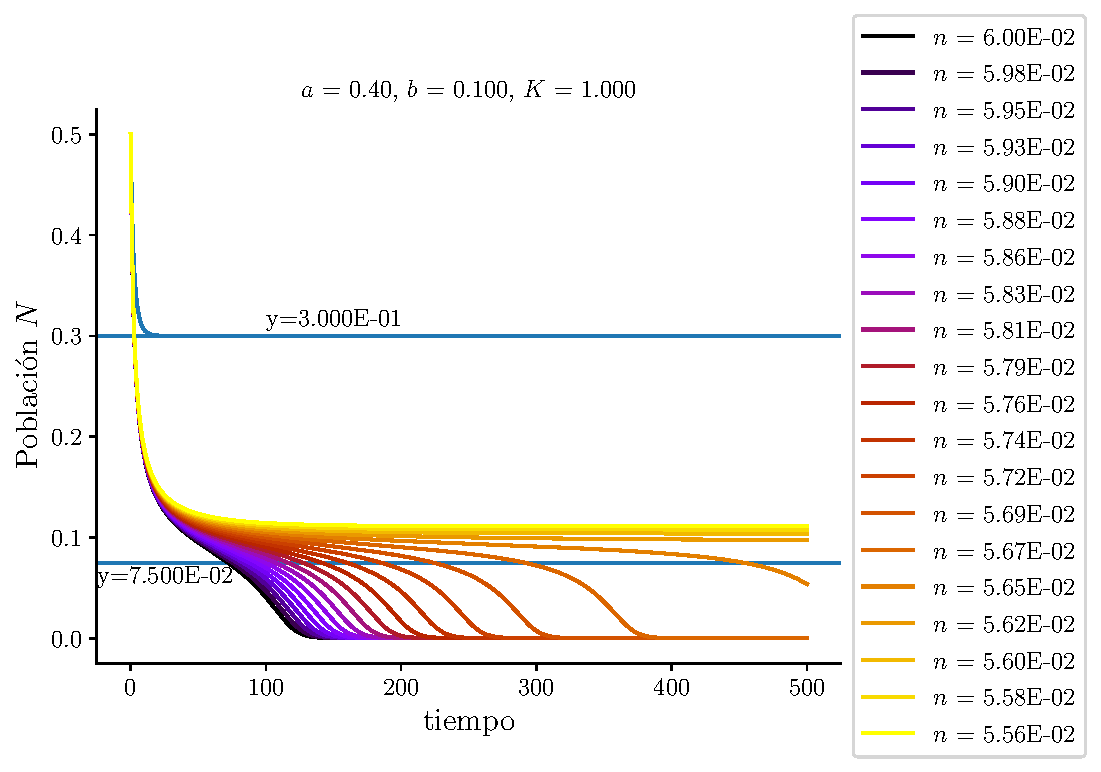
\includegraphics[width=0.55\textwidth]{figuras/ex5.pdf}
    \caption{Evolucion de los mosquitos fertiles para distintos valores de los mosquitos esteriles.}
    \label{fig:mosquitos}
\end{figure}

% 
% ███████╗██╗  ██╗    ██████╗     
% ██╔════╝╚██╗██╔╝    ╚════██╗    
% █████╗   ╚███╔╝      █████╔╝    
% ██╔══╝   ██╔██╗      ╚═══██╗    
% ███████╗██╔╝ ██╗    ██████╔╝    
% ╚══════╝╚═╝  ╚═╝    ╚═════╝     
%                                 
% 

\section{Resolucion Ej 3:}

Para el siguiente sistema de competencia ciclica:
$$
\begin{aligned}
\frac{d n_{1}}{d t}&=n_{1}\left(1-n_{1}-\alpha n_{2}-\beta n_{3}\right) = f_1(n_1,n_2,n_3)\\
\frac{d n_{2}}{d t}&=n_{2}\left(1-\beta n_{1}-n_{2}-\alpha n_{3}\right) = f_2(n_1,n_2,n_3) \\
\frac{d n_{3}}{d t}&=n_{3}\left(1-\alpha n_{1}-\beta n_{2}-n_{3}\right) = f_3(n_1,n_2,n_3)
\end{aligned}
$$
con $0<\beta<1<\alpha$ y $\alpha+\beta>2$. Pueden obtenerse los  equilibrios viendo todos los puntos que cumplan simultaneamente: 

$$
\begin{aligned}
    f_1(\nstar_1,\nstar_2,\nstar_3) = 0\\ 
    f_2(\nstar_1,\nstar_2,\nstar_3) = 0\\ 
    f_3(\nstar_1,\nstar_2,\nstar_3) = 0   
\end{aligned}
$$

Son 8 puntos de equilibrios $P_j = (\nstar_{1,j},\nstar_{2,j},\nstar_{3,j}), j= 1, 3, ..., 8$.

$$
\begin{aligned}
    P_1 &= (0, 0, 0) \\ 
    P_2 &= (1, 0, 0) \\ 
    P_3 &= (0, 1, 0) \\ 
    P_4 &= (0, 0, 1) \\  
    P_5 &= \frac{1}{\alpha \beta - 1} 
                       (\alpha - 1, \beta - 1 , 0) \\ 
    P_6 &= \frac{1}{\alpha \beta - 1} 
                       (0         , \alpha - 1, \beta - 1) \\ 
    P_7 &= \frac{1}{\alpha \beta - 1} 
                       (\beta - 1 , 0         , \alpha - 1) \\ 
    P_8 &= \frac{1}{\alpha + \beta + 1}(1, 1, 1) 
\end{aligned}
$$

Analizamos el la matriz jacobiana de este sistema:

% $$
% \mathbf{J} = 
% \begin{bmatrix}
%     1 - 2 x - \alpha y - \beta z & - \alpha x & - \beta x \\
%     - \beta y & 1 - 2 y - \beta x - \alpha z & - \alpha y \\
%     - \alpha z & - \beta z & 1 - \alpha x - \beta y - 2 z
% \end{bmatrix}
% $$

$$
\mathbf{J}_5 = 
\begin{bmatrix}
    -\talf  & - \alpha (\talf)& - \beta (\talf)\\
    - \beta (\tbet) & -\tbet & - \alpha (\tbet) \\
    0 & 0 & 1 - \alpha (\talf) - \beta (\tbet)
\end{bmatrix}
$$

$$
\mathbf{J}_6 = 
\begin{bmatrix}
    1 - \alpha (\talf) - \beta (\tbet) & 0 & 0 \\
    - \beta (\talf) & -\talf & - \alpha (\talf) \\
    - \alpha (\tbet) & - \beta (\tbet) & \tbet
\end{bmatrix}
$$

$$
\mathbf{J}_7 = 
\begin{bmatrix}
    -\tbet & - \alpha (\tbet) & - \beta (\tbet) \\
    0 & 1 - \beta (\tbet) - \alpha (\talf) & 0 \\
    - \alpha (\talf) & - \beta (\talf) & \talf
\end{bmatrix}
$$


$$
\mathbf{J}_1 = 
\begin{bmatrix}
    1  & 0 & 0 \\
    0 & 1 & 0 \\
    0 & 0 & 1
\end{bmatrix}
\quad 
\mathbf{J}_8 = 
\frac{1}{1+\alpha+\beta}\begin{bmatrix}
    -1 & -\alpha & -\beta \\
    -\beta & -1 & -\alpha \\
    -\alpha & -\beta & -1
\end{bmatrix}
$$

$$
\mathbf{J}_2 = 
\begin{bmatrix}
    -1 & - \alpha & - \beta \\
    0 & 1-\beta & 0 \\
    0 & 0 & 1- \alpha
\end{bmatrix}
$$

$$
\mathbf{J}_3 = 
\begin{bmatrix}
    1 - \alpha  & 0 & 0 \\
    - \beta & -1 & - \alpha \\
    0 & 0 & 1  - \beta
\end{bmatrix}
,
\mathbf{J}_4 = 
\begin{bmatrix}
    1 - \beta  & 0 & 0 \\
    0 & 1 -\alpha  & 0 \\
    - \alpha  & -\beta & -1
\end{bmatrix}
$$



El origen es equilibrio (una fuente) y los versores $(1,0,0)$ etc. son puntos de ensilladura. Hay otros 3 equilibrios con dos poblaciones finitas y una nula. Finalmente, existe un equilibrio interior al octante $\mathbb{R}_{+}^{3}$, dado por:
$$
x_{1}^{*}=x_{2}^{*}=x_{3}^{*}=\frac{1}{1+\alpha+\beta} .
$$
Este equilibrio de coexistencia es una ensilladura, lo cual se demuestra fácilmente porque los autovalores son muy sencillos. La matriz del sistema linealizado es "circulante":
$$
\frac{1}{1+\alpha+\beta}\left(\begin{array}{ccc}
-1 & -\alpha & -\beta \\
-\beta & -1 & -\alpha \\
-\alpha & -\beta & -1
\end{array}\right)
$$
con lo que sus autovalores son combinaciones de las raíces cúbicas de la unidad:
$$
\lambda_{k}=\sum_{j=0}^{n-1} c_{j} \gamma_{j}^{k}, \quad k=0,1, \ldots, n-1
$$
con $c_{j}$ los elementos de la matriz y $\gamma_{j}$ las raíces de la unidad, $\gamma_{j}=\exp (2 \pi i / n)$, en general. Así que:
$$
\begin{array}{c}
\lambda_{0}=-1, \text { con autovector }(1,1,1) \\
\lambda_{1}=\lambda_{2}^{*}=\frac{1}{1+\alpha+\beta}\left(-1-\alpha e^{2 x i / 3}-\beta e^{4 \pi i / 3}\right),
\end{array}
$$
que satisfacen:
$$
\operatorname{Re}\left(\lambda_{1}\right)=\operatorname{Re}\left(\lambda_{2}\right)=\frac{1}{1+\alpha+\beta}\left(-1+\frac{\overbrace{\alpha+\beta}^{>2}}{2}\right)>0
$$

% 
% ███████╗██╗  ██╗    ██╗  ██╗
% ██╔════╝╚██╗██╔╝    ██║  ██║
% █████╗   ╚███╔╝     ███████║
% ██╔══╝   ██╔██╗     ╚════██║
% ███████╗██╔╝ ██╗         ██║
% ╚══════╝╚═╝  ╚═╝         ╚═╝
%                             
% 

\section{Resolucion Ej 4:}

El sistema de ecuaciones
$$
\begin{aligned}
\frac{d x}{d t} = f_1(x, y, z) &=-c_{a} x y+e_{a} y-c_{b} x z+e_{b} z \\
\frac{d y}{d t} = f_2(x, y, z) &=c_{a} x y-e_{a} y+c_{a} z y          \\
\frac{d z}{d t} = f_3(x, y, z) &=c_{b} x z-e_{b} z-c_{a} z y            
\end{aligned}
$$

Los equilibrios vienen dados por 

$$
\begin{aligned}
    f_1(x^*, y^*, z^*) = 0\\ 
    f_2(x^*, y^*, z^*) = 0\\ 
    f_3(x^*, y^*, z^*) = 0   
\end{aligned}
$$

Por esto los puntos fijos son:

$$
\begin{aligned}
    P_1 &= (0, 0, 0) \\ 
    P_2 &= (\frac{e_b}{c_b}, 0, z) \\ 
    P_3 &= (\frac{e_a}{c_a}, y, 0) \\ 
    P_4 &= (\frac{e_a}{c_a} - c_a z, z, \frac{c_b}{c_a} (\frac{e_a}{c_a} - c_a z) - \frac{e_b}{c_a}) 
\end{aligned}
$$


$$
J = 
\begin{bmatrix}  
    - y c_a - z c_b & - x c_a + e_a & - x c_b + e_b \\
    y c_a & x c_a - e_a + z c_a & y c_a \\
    z c_b & - z c_a & x c_b - e_b - y c_a 
\end{bmatrix}
$$

$$
J_1 = 
\begin{bmatrix}
    0 & e_a & e_b \\
    0 & - e_a & 0 \\
    0 & 0 & - e_b 
\end{bmatrix}
$$

$$
J_2 = 
\begin{bmatrix}  
    - z c_b & - (\frac{e_b}{c_b}) c_a + e_a & - (\frac{e_b}{c_b}) c_b + e_b \\
    0 & (\frac{e_b}{c_b}) c_a - e_a + z c_a & 0 \\
    z c_b & - z c_a & (\frac{e_b}{c_b}) c_b - e_b
\end{bmatrix}
$$


$$
J = 
\begin{bmatrix}  
    - y c_a & - (\frac{e_a}{c_a}) c_a + e_a & - (\frac{e_a}{c_a}) c_b + e_b \\
    y c_a & (\frac{e_a}{c_a}) c_a - e_a  & y c_a \\
    0 & 0 & (\frac{e_a}{c_a}) c_b - e_b - y c_a 
\end{bmatrix}
$$

% 
% ███████╗██╗  ██╗    ███████╗
% ██╔════╝╚██╗██╔╝    ██╔════╝
% █████╗   ╚███╔╝     ███████╗
% ██╔══╝   ██╔██╗     ╚════██║
% ███████╗██╔╝ ██╗    ███████║
% ╚══════╝╚═╝  ╚═╝    ╚══════╝
%                             
% 

\section{Resolucion Ej 5:}

% 
% ███████╗██╗  ██╗     ██████╗ 
% ██╔════╝╚██╗██╔╝    ██╔════╝ 
% █████╗   ╚███╔╝     ███████╗ 
% ██╔══╝   ██╔██╗     ██╔═══██╗
% ███████╗██╔╝ ██╗    ╚██████╔╝
% ╚══════╝╚═╝  ╚═╝     ╚═════╝ 
%                              
% 

\section{Resolucion Ej 6:}

\bibliography{sample}

\end{document}

% ███    ██  ██████  ████████  █████  ███████
% ████   ██ ██    ██    ██    ██   ██ ██
% ██ ██  ██ ██    ██    ██    ███████ ███████
% ██  ██ ██ ██    ██    ██    ██   ██      ██
% ██   ████  ██████     ██    ██   ██ ███████


% ████████ ██    ██ ██████   ██████  ███████
%    ██     ██  ██  ██   ██ ██    ██ ██
%    ██      ████   ██████  ██    ██ ███████
%    ██       ██    ██      ██    ██      ██
%    ██       ██    ██       ██████  ███████

% A pesar de mis multiples y cultas intervenciones seguis escribiendo así, usa ctrl f y resolvelo.

% atomico
% volumen
% parametro
% mantenia
% dielectrico
% perdida
% ferroelectrico
% difractograma
% difractometro
% minimo
% maximo
% tension
% conversion
% aislacion
% medicion
% resolucion
% funcion
% transicion
% correccion
% activacion
% correlacion
% tipico X
% habia  X
% agrego X
